\documentclass{article}

\usepackage{tabularx}

% NOTE: To put equations in their environment we need either `float` or
% `caption`.  We use float to put equations and other environments exactly
% where they appear in the code with the `H` placeholder, and for that we
% redefine the `equ` environment sort of twice, so this is a bit flaky but
% it works.
\usepackage{caption}
\DeclareCaptionType{equ}[][]
\captionsetup[equ]{name=נוסחא}
\usepackage{float}
\floatstyle{plain}
% https://www.overleaf.com/learn/latex/Positioning_of_Figures
\newfloat{equ}{H}{eq}[section]
\floatname{equ}{נוסחא}

\DeclareCaptionType{graph}[][]
\captionsetup[graph]{name=גרף }

% to includegraphics
\usepackage{graphicx}

% to fix itemize lists:
% https://tex.stackexchange.com/a/53453/125609
\usepackage{enumitem}
\setlist[itemize,1]{label={\fontfamily{cmr}\fontencoding{T1}\selectfont\textbullet}}

% Links
\usepackage{hyperref}
\hypersetup{colorlinks = true,
	citecolor = gray,
	linkcolor = red,
	citecolor = green,
	filecolor = magenta,
	urlcolor = cyan
}

% To include plots by matplotlib
\usepackage{pgfplots}
\pgfplotsset{compat=newest}
% Note we use resizebox as explained here through out the document https://tex.stackexchange.com/a/582956/125609
\usepackage{geometry}
 \geometry{
 a4paper,
 top=30mm,
 left = 25mm,
 right = 25mm,
 bottom=30mm,
 headheight=2cm,
 headsep=2cm,
 footskip=1.5cm
}
% Language
\usepackage{polyglossia}
\setdefaultlanguage{hebrew}
\setotherlanguage{english}
\usepackage{hebrewcal}

\usepackage[
backend=biber,
isbn=false,
style=numeric,
doi = false,
sorting=ynt
]{biblatex}
% Seems to be a recommended package but it makes quotes in bibliography at the
% end appear with a question mark instead of `"`.
%\usepackage{csquotes}
\addbibresource{references.bib} % Imports bibliography file

% Fonts
\setmainfont{David CLM}
\setsansfont{Liberation Sans}
\setmonofont{Liberation Mono}
\newfontfamily\hebrewfont{David CLM}[Script=Hebrew]
\newfontfamily\hebrewfontsf{Liberation Serif}[Script=Hebrew]
\newfontfamily\hebrewfonttt{Liberation Mono}[Script=Hebrew]

\title{
שימוש באפקט
\textenglish{Hall}
למדידת פער אנרגטי בין רמות אנרגיה ואישוש תאוריית שני נושאי מטען במוליך למחצה מסוג
\textenglish{n-Germanium}
}
\author{
שרה לחצר ודורון בכר \\
הפקולטה לפיזיקה, הטכניון - מכון טכנולוגי לישראל.
}
\date{\today}

\begin{document}
\maketitle

\begin{abstract}
בניסוי זה חקרנו את אפקט הול במוליך למחצה מסוג גרמניום 
$n-type$
בעזרת המערכת
\textenglish{Halleffect-Modul}
של חברת
\textenglish{PHYWE}.
ביצענו מדידות של מתח הול והמתח הישר כתלות בשינוי השדה המגנטי, הזרם העובר במוליך וטמפרטורת המוליך. 
מתוך המדידות חישבנו את הפער האנרגטי והראנו שבטמפרטורות גבוהות ניתן להתייחס למל"מ המסומם כאינטרינזי.
בנוסף חישבנו את המוביליות של נושאי המטען
והסקנו שחישוב המוביליות תחת הנחת נושא מטען יחיד איננה מדוייקת.

\end{abstract}
\section{מבוא}
\subsection{אפקט הול}
אפקט הול הוא תופעה פיזיקלית בה נוצר מתח חשמלי במוליך בכיוון הניצב לזרם העובר בו כתוצאה משדה מגנטי הניצב לשניהם. השדה המגנטי יוצר כוח על נושאי המטען שכיוונו ניצב לזרם ונוצרת הצטברות מטען שלילי בקצה אחד של המוליך ומטען חיובי בקצה המנוגד. כתוצאה מכך יווצר שדה חשמלי שיבטל את הכח שיוצר השדה המגנטי.
במצב זה, המתח הנמדד בניצב לזרם- מתח הול- נתון בנוסחא
\ref{equ:V_hall}.
בנוסף ניעזר בנוסחא 
\ref{equ:R_hall} 
המציגה את הקשר בין מוביליות נושאי המטען לגודל המכונה מקדם הול.

\begin{equ}
$$U_H = \frac{IB}{n e d}$$
\caption{מתח הול כתלות בזרם 
$I$,
השדה המגנטי
$B$,
צפיפות נושאי המטען
$n$,
ובמרחק בין קצוות המוליך בכיוון שדה הרוחבי
$d$.}
\label{equ:V_hall}
\end{equ}

\begin{equ}
$$\mu = R_H \sigma_0$$
\caption{מוביליות נושאי המטען כתלות 
במקדם הול -
$R_H = \frac{1}{ne}$
ו
$\sigma_0$
המוליכות החשמלית.}
\label{equ:R_hall}
\end{equ}


\subsection{מוליכים למחצה}

מוליכים למחצה הם חומרים מהטור הרביעי של הטבלה  המאופיינים ב-4 אלקטרוני ערכיות. כאשר החומר מסודר כגביש טהור, כל אטום בשריג הגבישי הוא בעל 4 שכנים איתם הוא נמצא בקשר קוולנטי, כך שלמעשה בכל המערכת אין אלקטרונים חופשיים להולכה. גביש כזה נקרא מוליך למחצה אינטרינזי.
על מנת להגדיל את ההולכה של המל"מ מבצעים אילוח
על ידי הוספה של חומרים מהעמודה החמישית או השלישית.
בעת הוספת חומרים מהעמודה החמישית נוספים אלקטרונים עודפים למערכת, ואילו בעת הוספת  חומרים מהעמודה השלישית נוצרים קשרים קוולנטיים בהם חסר אלקטרון.
מחסור בקשר הקוולנטי באלקטרון נקרא חור והוא מתנהג כמו נושא מטען חיובי.

במל"מ אינטרינזי בשיווי משקל סה"כ ריכוז החורים קבוע וריכוז אלק' קבוע כי בממוצע על כל אלק' שעולה לפס
ההולכה ויוצר חור, יש אחד שיורד לרמת הערכיות וממלא חור.

\clearpage

אפקט הול במל"מ מאופיין ע"י שני נושאי מטען- חורים ואלקטרונים- לכן נצטרך להרחיב את נוסחאות 
\ref{equ:R_hall}
ו-
\ref{equ:V_hall}
לשני נושאי מטען.
מקדם הול עבור שני נושאי מטען נתון בנוסחא 
\ref{equ:R_hall_2_carriers}
והקשר בין המתח הישר , השדה המגנטי והזרם עבור שני נושאי מטען נתון בנוסחא
\ref{equ:V_2_carriers}.


\begin{equ}
$$R_H = \frac{\mu_h^2 p-\mu_e^2 n}{e(\mu_h p-\mu_e n)^2}$$
\caption{
מקדם הול עבור שני נושאי מטען כאשר 
$\mu_{e/h}$, ${n/p}$ -
מוביליות וצפיפות האלקטרונים/חורים בהתאמה.
}
\label{equ:R_hall_2_carriers}
\end{equ}

\begin{equ}
$$U_p = (\frac{1}{e(\mu_h p-\mu_e n)}+
B^2\frac{\mu_h p \mu_e n(\mu_h +\mu_e)^2}{e(\mu_h p-\mu_e n)^3})
\frac{I \cdot l}{A}$$
\caption{
המתח האורכי
$U_p$
עבור שני נושאי מטען כאשר 
$\mu_{e/h}$, ${n/p}$ -
מוביליות וצפיפות האלקטרונים/חורים בהתאמה ו-
$B$
השדה המגנטי.
}
\label{equ:V_2_carriers}
\end{equ}

גורם נוסף שיכול להשפיע על ההולכה של חומר היא הטמפרטורה, סכימה תאורטית שמציגה את ההשפעה מוצגת בגרף
\ref{fig:conductivity_temp_theory}.

% TODO: add ref to guide
\begin{graph}[H]
    \centering
    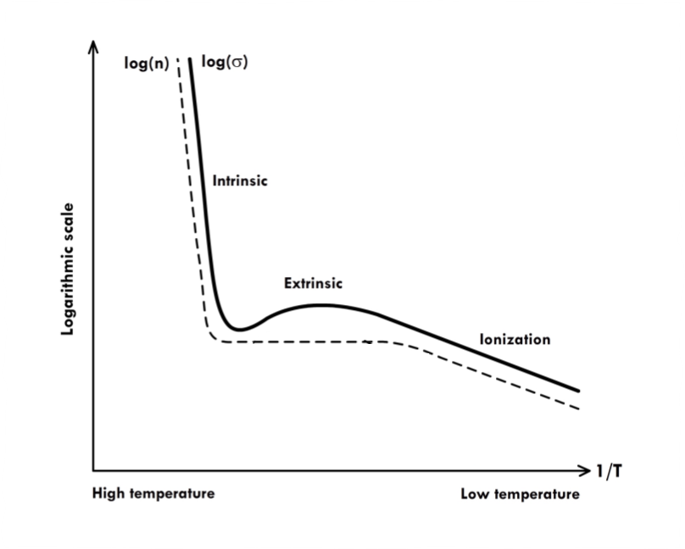
\includegraphics[width=0.8\textwidth]{Hall_temp.png}
    \caption{
    מוליכות, מוביליות וצפיפות נושאי המטען כתלות בטמפרטורה,
    לקוח מהתדריך
    \cite{Manual}.
    }
    \label{fig:conductivity_temp_theory}
\end{graph}

בטמפ' מאוד נמוכות,
נושאי המטען של החומר המסמם עוד מחוברים לאטומי
האילוח ואינם חופשיים לנוע בשריג בפס
ההולכה. עם העליה בטמפ' אטומי האילוח
יעברו יינון והאלקטרונים שלהם יעברו
לפס ההולכה. 
בתחום האקסטרינזי כל נושאי המטען של החומר המסמם יהיו מיוננים וכמות נושאי המטען בקירוב נשארת קבועה.
לבסוף, בטמפרטורות הגבוהות מסופקת למערכת מספיק אנרגיה להתגבר על הפער האנגטי של המלמ והחומר המסמם נהיה זניח.
בתחום זה המל"מ נהיה אינטרינזי והקשר בין כמות נושאי המטען לטמפרטורה נתון בנוסחא 
\ref{fig:conductivity_temp_theory}.

\begin{equ}
$$n = n_0 e^{-\frac{E_g}{2 K_b T}}$$
\caption{
כמות נושאי המטען כתלות בטמפרטורה עבור מל"מ אינטרינסי.
}
\label{equ:n_temp_intrinsic}
\end{equ}

בניסוי זה נעבוד עם מערכת של 
\textenglish{PHYWE}-
\textenglish{Halleffect-Modul},
עם המל"מ
\textenglish{germanium}
מסוג 
\textenglish{n-type}.

\section{תוצאות}

בחלקו הראשון של הניסוי מדדנו את המתח האורכי
$U_p$
כתלות בזרם האורכי
$I$
בלי שדה מגנטי, בכוונה למצוא את ההתנגדות
$R_0$
מחוק
אוהם
שתשמש אותנו בהמשך.
התוצאות מוצגות בגרף
\ref{fig:part_0}.

\begin{graph}[H]
    \centering
    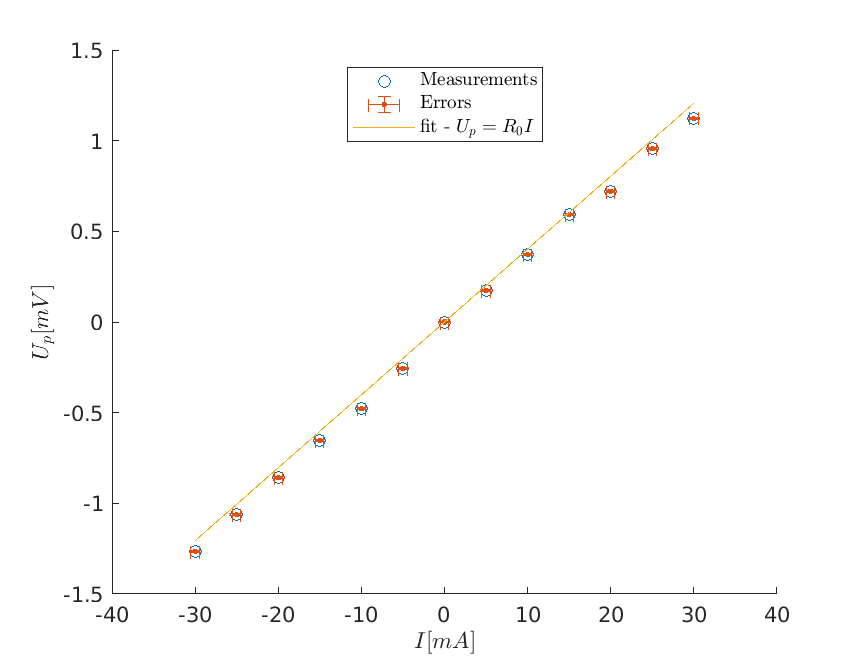
\includegraphics[width=0.7\textwidth]{part0 - R_0.png}
    \caption{
    מציאת ההתנגדות
    $R_0$
    באמצעות חוק אוהם.
    }
    \label{fig:part_0}
\end{graph}

קיבלנו ש-
$R_0 = 40 \pm 2 \Omega$
כאשר בהתאמה למודל הלינארי קיבלנו טיב התאמה של
$R^2 = 0.9946$.

לאחר מדידה זו, הפעלנו שדה מנגטי בניצב לכיוון הזרם בעוצמה של 
$B = (250 \pm 1) mT$ 
לשם קבלת אפקט הול. ביצענו התאמה בהתאם לנוסחא
\ref{equ:V_hall},
התוצאות מוצגות בגרף
\ref{fig:part_1}.
\begin{graph}[H]
    \centering
    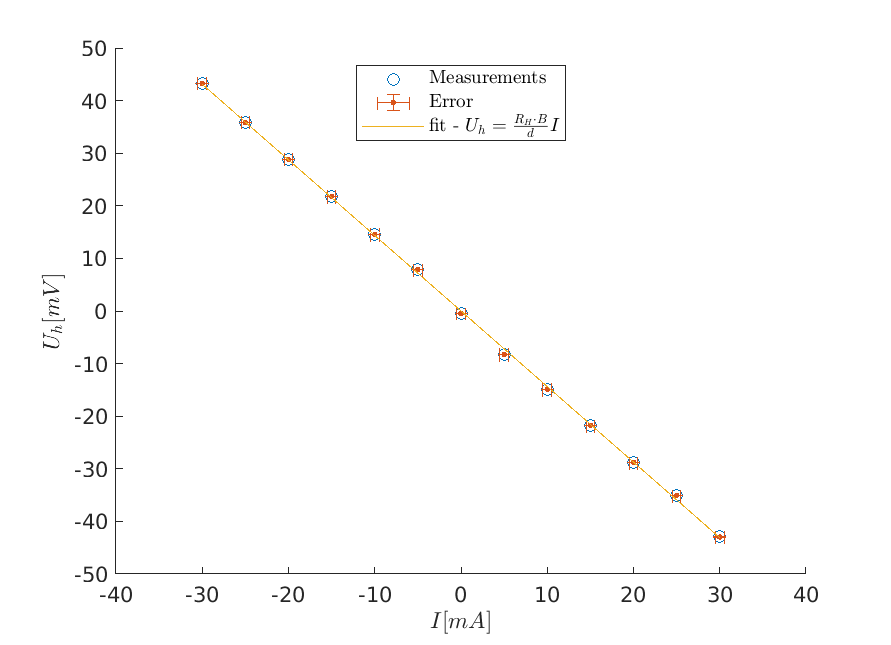
\includegraphics[width=0.7\textwidth]{part1 - R_h.png}
    \caption{מתח הול כתלות בזרם}
    \label{fig:part_1}
\end{graph}


במדידה זו קיבלנו טיב התאמה של
$R^2 = 0.9997$
וקיבלנו מקדם הול
$R_h = -7.38 \pm 0.01 [\frac{\Omega m}{T}]$.
השתמשנו בנוסחא
\ref{equ:R_hall}
וחישבנו את מוביליות נושאי המטען 
$\mu = -0.29 \pm 0.01 [\frac{m^2}{V sec}] $,
כאשר הנחנו שהאלקטרון הוא נושא המטען הדומיננטי והזנחנו את החורים כפי שהוצע ב
\cite{Manual}.

לאחר מכן קבענו זרם קבוע של
$I = (30 \pm 1) mA$,
שינינו את השדה המגנטי
ומדדנו את מתח הול ואת המתח הישר במערכת.
בגרף
\ref{fig:part_2}
מוצגות מדידות של מתח הול כתלות בשדה המגנטי
בהתאם לנוסחא
\ref{equ:V_hall}.
בגרף
\ref{fig:part_3}
מוצגות מדידות של המתח האורכי
בהתאם לנוסחא
\ref{equ:V_2_carriers}.

\begin{graph}[H]
    \centering
    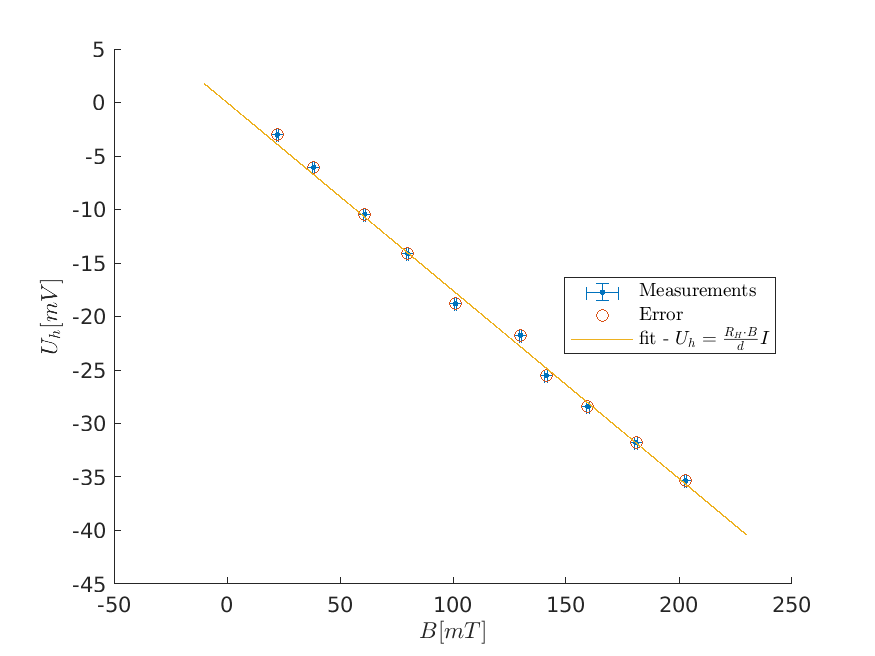
\includegraphics[width=0.7\textwidth]{part2 - R_h.png}
    \caption{מתח הול כתלות בשדה המגנטי}
    \label{fig:part_2}
\end{graph}

במדידה 
\ref{fig:part_2}
קיבלנו טיב התאמה של
$R^2 = 0.9962$
וקיבלנו מקדם הול
$R_h = -6.31 \pm 0.01 [\frac{\Omega m}{T}]$.
גם כאן חישבנו את מוביליות נושאי המטען וקיבלנו כי 
$\mu = -0.25 \pm 0.01 [\frac{m^2}{V sec}]$,
תחת ההנחה שנושאי המטען הדומיננטים הם האלקטרונים.

במדידה
\ref{fig:part_3}
חישבנו את המתח האורכי
$U_p$
כתלות בשדה המגנטי וקיבלנו התנהגות דומה להתנהגות המתוארת בנוסחא
\ref{equ:V_2_carriers}.
ביצענו התאמה לפולינום זוגי מסדר שני וקיבלנו התאמה של
$R^2 = 0.999$
למודל.


%nt_part2_fitresult = 
%       p1 =     -0.1758  (-0.1796, -0.1719)
%nt_part2_gof = 
%       rsquare: 0.9962
%nt_part2_R_h =
%   -0.0059
%nt_number_of_charges =
%  -1.0655e+21
%nt_part2_mu =
% -233.1553


\begin{graph}[H]
    \centering
    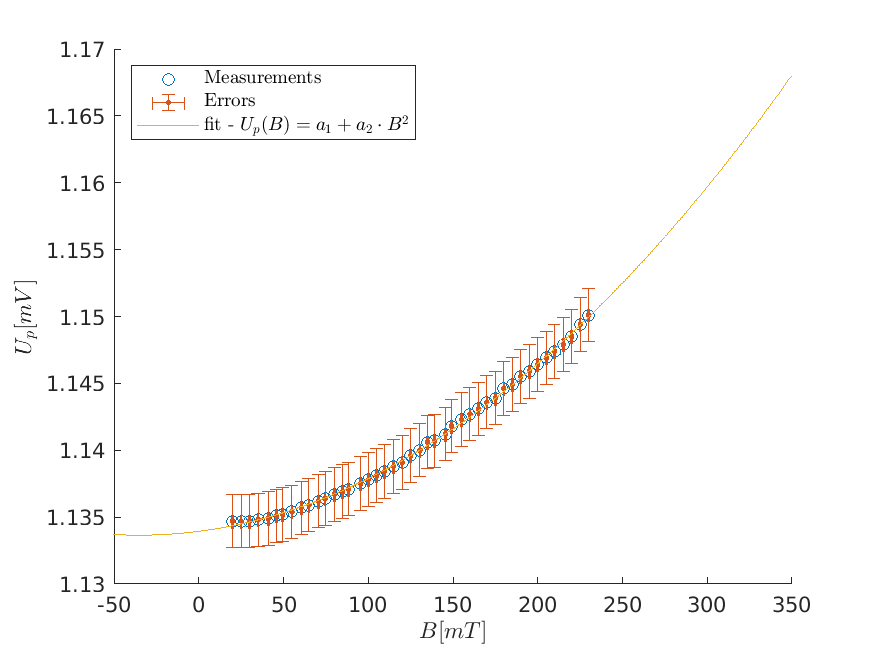
\includegraphics[width=0.7\textwidth]{part3 - B-squared relation.png}
    \caption{המתח האורכי כתלות בשדה המגנטי}
    \label{fig:part_3}
\end{graph}

לבסוף מדדנו את הקשר בין המוליכות לטמפרטורה בעזרת שתי מדידות: מדידת המתח האורכי
$U_p$
ומתח הול
$U_h$
כתלות בטמפרטורה.
התוצאות מוצגות בגרפים
\ref{fig:part_4}
ו-
\ref{fig:part_5}
בהתאמה.

\begin{graph}[H]
    \centering
    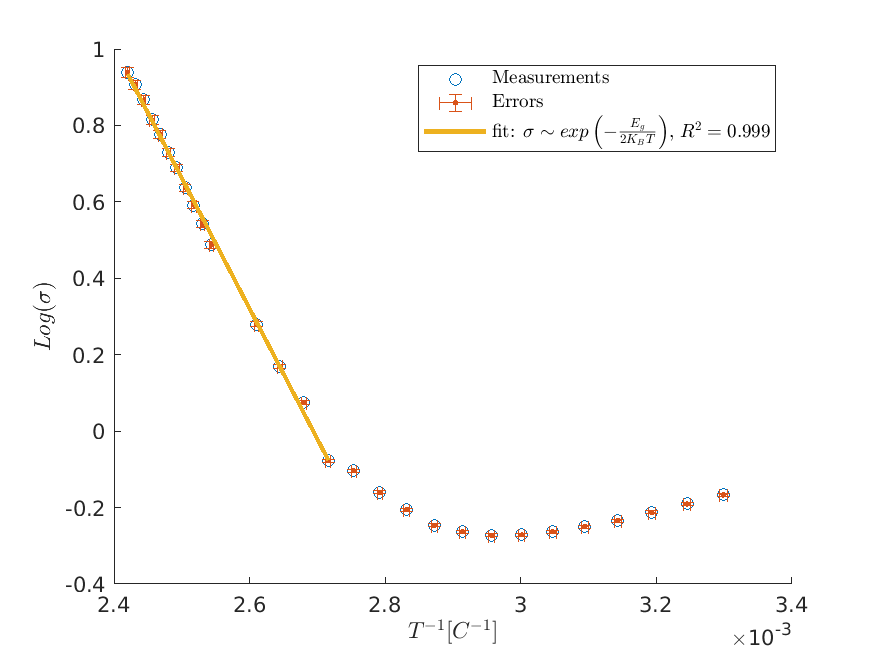
\includegraphics[width=0.8\textwidth]{part4 - E_g.png}
    \caption{
    מוליכות כתלות בטמפרטורה במדידת מתח אורכי
    }
    \label{fig:part_4}
\end{graph}

%nt_part4_fitresult = 
%       p1 =       -3416  (-3499, -3333)
%       p2 =       9.201  (8.991, 9.411)
%nt_part4_gof = 
%       rsquare: 0.9984
%nt_part4_energy_gap =
%   -0.5892

\begin{graph}[H]
    \centering
    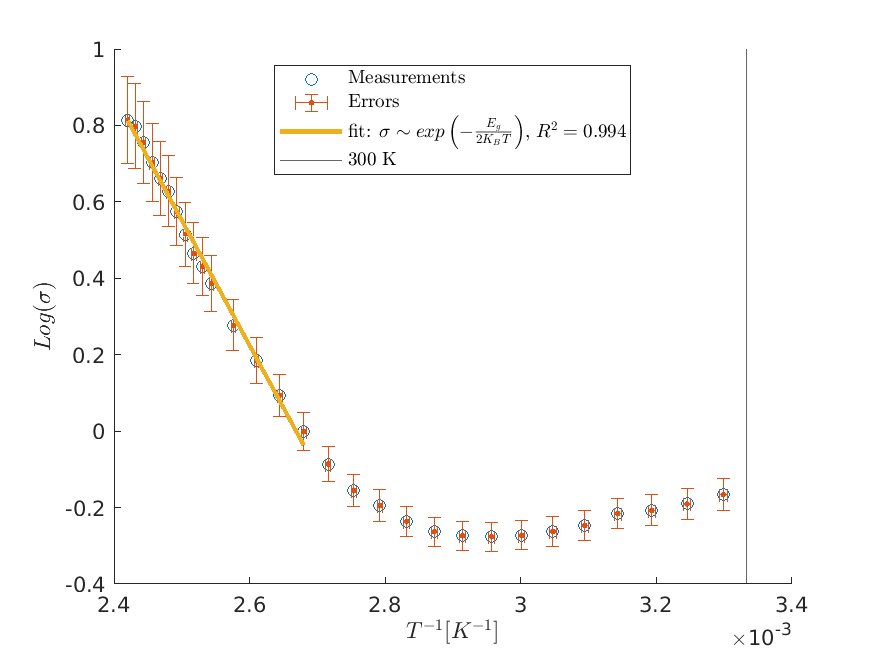
\includegraphics[width=0.8\textwidth]{part5 - E_g with magnetic field.png}
    \caption{
    מוליכות כתלות בטמפרטורה במדידת מתח הול
    }
    \label{fig:part_5}
\end{graph}

ביצענו את ההתאמה בהתאם לנוסחא
\ref{equ:n_temp_intrinsic},
כך חישבנו את הפער האנרגטי בין פסי ההולכה במל"מ, וקיבלנו
$E_g = 0.58 \pm 0.01[eV]$
ו-
$E_g = 0.56 \pm 0.02[eV]$
בהתאם לגרפים
\ref{fig:part_4}
ו-
\ref{fig:part_5}
בהתאמה.
% TODO: Reference \cite{ManufacturerManual}.
\section{דיון בתוצאות}
תחילה חישבנו את ערך ההתנגדות של הנגד בעזרת מדידה פשוטה של חוק אוהם, ראינו שהערך עומד במבחן רווח בר סמך והשתמשנו בו בחישובים בהמשך.


ביצענו שתי מדידות שונות עבור
$R_h$,
הראשונה בעזרת שינוי הזרם והשנייה בעזרת שינוי השדה המגנטי.
השתמשנו בערכי ה
$R_h$
בכדי לחשב את המוביליות תחת ההנחה שהאלקטרונים הם נושאי המטען הדומיננטיים ושהחורים זניחים.
השוונו את הערכים אל מול ערכי היצרן, קיבלנו כי הערך שהתקבל מגרף
\ref{fig:part_1}
איננו עומד במבחן רווח בר סמך ובעל שגיאה של 
$16\%$
מערך היצרן.
לעומת זאת מתוך המדידות שהתקבלו בגרף 
\ref{fig:part_2}
הצלחנו לקבל התאמה טובה יותר והן עמדו במבחן רווח בר-סמך אל מול ערכי היצרן.

תחילה נציין כי ערכי המוביליות שמדדנו וערך המובליות שסיפק היצרן כולם נמדדו בעזרת אפקט הול במוליכים למחצה, לכן זוהי אינה דרך לבחינת התוצאות.
בנוסף, היצרן לא סיפק את אופן הסימום כלומר את אחוז החומר המסמם במלמ,
לכן גם אם היינו רוצים להשוות בדרך כלשהי את התוצאות לא הייתה לנו אפשרות לכך.


באשר לשגיאה שקיבלנו עבור מדידת מתח הול כתלות בשדה המגנטי- הבחנו בעת הניסוי שהשדה אינו קבוע ואנו סבורים כי הוא מקור השגיאה. 

לאחר מכן מדדנו את המתח הישר כתלות בשדה המגנטי תחת ההנחה שיש שני נושאי מטען.
הן מבחינה ויזואלית והן מבחינה כמותית ראינו שאכן יש התאמה בין נוסחא
\ref{equ:V_2_carriers}
לבין תוצאות המדידה. מכאן הסקנו שהנחת שני נושאי המטען מתאימה במערכת, למרות כי ייתכן שאחד מהם דומיננטי יותר.
רצינו לבחון אם ההנחה שביצענו בחישוב המוביליות (נושא מטען יחיד)
הייתה תקפה.
חשבנו שייתכן שהגודל הקטן
$\frac{p}{n}$
מופיע בסדרים גדולים יותר בנוסחא
\ref{equ:R_hall_2_carriers}
לעומת במקדם של 
$B^2$
בנוסחא
\ref{equ:V_2_carriers}
ועל כאן האפקט של שני נושאי המטען זניח בנוסחא
\ref{equ:R_hall_2_carriers}.
וקיבלנו ש
$\frac{p}{n}$
מופיע בסדר ראשון בשתי הנוסחאות לכן אנו סבורים שההנחה שביצענו בחישוב המוביליות לא הייתה טובה.

לאחר מכן בחנו את ערכי פערי האנרגיה שהתקבלו,
בבאנו להשוות אותם מול ערכי היצרן הבחנו שיש שגיאת חישוב בסדר גודל בערכים שפרסם היצרן.
חישבנו מתוך נתוני היצרן את הערך של פער האנרגיה וקיבלנו שגיאה של 
$16\%$
מהערך של היצרן.
גם כאן לא הייתה לנו אפשרות להשוות את הערכים מול ערך תאורטי כיוון שלא ידענו את הרכב המל"מ.
אך הצלחנו להראות שיש התאמה טובה בתחום הטמפרטורות הגבוהות למל"מ אינטרינזי.

\section{מסקנות}

הצלחנו למדוד את הפער האנרגטי בין פסי ההולכה במל"מ ואת ריכוז נושאי המטען לפי מודל דרודה ובאמצעות אפקט הול. אנו סבורים שלא ניתן להעריך את ערכים אלו לפי תכונות החומר כגון הסימום שלו. על אף זאת, קיבלנו מקדם הול
$R_H$
שלילי כמצופה ממל"מ מסוג
\textenglish{n-type}.
הדגמנו את התוצאות המתקבלות ממודל דרודה ומאפקט הול, והסקנו שלא ניתן לחשב ממדידות אלו את ריכוז שני נושאי המטען ואת המוביליות של שני נושאי המטען.

\section*{סימוכין}
\begin{english}
\printbibliography[heading=none]{}
\end{english}

\end{document}